\documentclass[c]{beamer}

\usepackage[utf8]{inputenc}
\usepackage[francais]{babel}

% figures
\setbeamerfont{caption}{size=\tiny}

% margins
\setbeamersize{text margin left=3em, text margin right=3em}

% puces
\setbeamertemplate{itemize item}[ball] % Pour le premier niveau
\setbeamertemplate{itemize subitem}[triangle] % Pour le deuxième niveau
\setbeamertemplate{itemize subsubitem}[circle] % Pour le troisième niveau

% links
\definecolor{links}{HTML}{2A1B81}
\hypersetup{colorlinks,linkcolor=,urlcolor=links}

% theme
\usetheme{Warsaw}


\title[High-Res satellite images for human density prediction]{High-Res Landsat-8 satellite images \\for human density prediction}

\author{Youcef Kacer}

\institute{www.github.com/ykacer}

\date{2017,January 25\textsuperscript{th}}

%color
\colorlet{rouge}{red} % rename colors in frencj
\colorlet{grisfonce}{darkgray}
\colorlet{titre}{yellow}
\definecolor{vertmoyen}{RGB}{51,110,23} % custom rgb color
\definecolor{rouge}{HTML}{DD0000} % custom html color

\begin{document}
\begin{frame}
\titlepage
\logo{\includegraphics[height=5mm]{images/logo/TelecomParisTech_logo_200_01.png}}
\end{frame}

\begin{frame}
\tableofcontents
\end{frame}

\section{Presentation}
\begin{frame}
\tableofcontents[currentsection]
\end{frame}

\begin{frame}
\begin{itemize}
\item Population census is expensive using conventional methods\\
  \begin{itemize}
  \item 180 millions euros in France (\href{http://www.assemblee-nationale.fr/13/rap-info/i1246.asp}{officials,1999})\\ 
  \end{itemize}
\item How High-resolution satellites images could explain human density?\\
\item How to transform HR satellite images to explain human density?\\
\end{itemize}
\end{frame}

\section{Landsat-8 imagery}

\subsection{Earth Covering}
\begin{frame}[label=Covering]
\tableofcontents[currentsubsection]
\end{frame}

\begin{frame}
\begin{itemize}
\item Total earth covering defined by path,row grid pattern and achieved every 16 days
\end{itemize}
\begin{figure}
  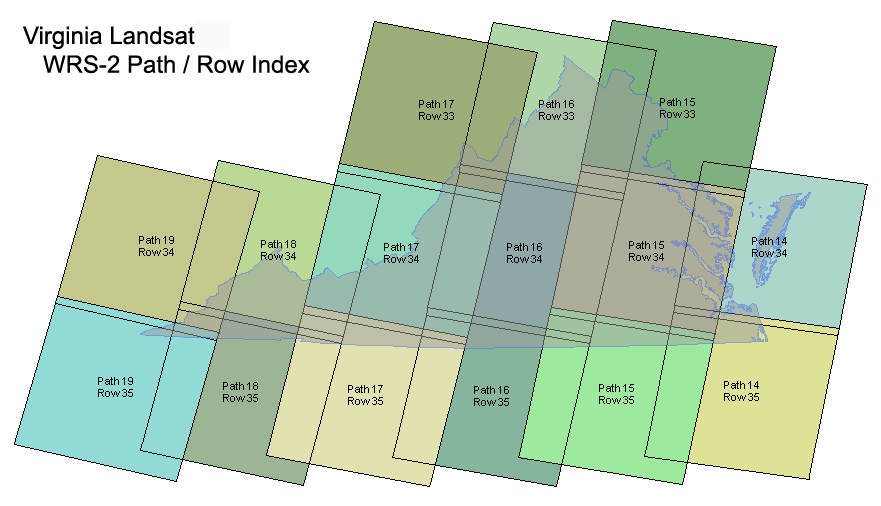
\includegraphics[scale=0.13]{images/covering/wrs.png}
  \caption{Landsat-8 grid covering (path,row) for Virginia ($USA$) }
\end{figure}
\end{frame}

\subsection{Image Georeferencement}
\begin{frame}
\tableofcontents[currentsubsection]
\end{frame}

\begin{frame}
\begin{itemize}
 \item Landsat-8 images are georeferenced which means each pixel has (x,y) meter coordinates in a certain Projection Coordinates 
System (\begin{itshape}ex: UTM, Lambert IV, Lambert 93, Web Mercator,...\end{itshape})
\end{itemize}
\begin{columns}

\begin{column}{5cm}
\begin{figure}
  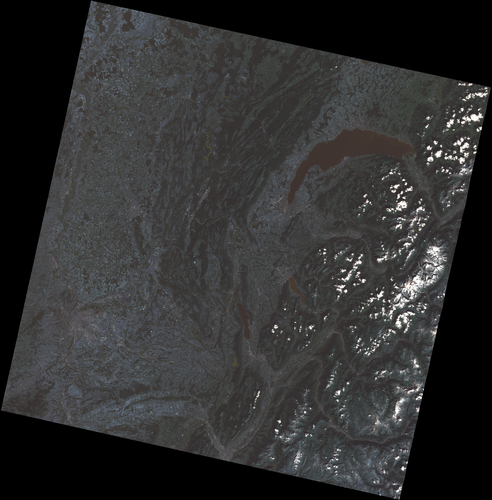
\includegraphics[scale=0.2]{images/georeferencing/Thonon_landsat.png}
  \caption{Landsat-8 Eastern-France image path=$196$,row=$028$ georeferenced in $UTM$ system (image containing city Thonon-les-Bains)}
\end{figure}
\end{column}

\begin{column}{5cm}
\begin{block}{coordinates}
 \begin{itemize}
  \item upper-left (,)\\
  \item upper-right (,)\\
  \item bottom-right (,)\\
  \item bottom-left (,)\\
  \item center (,)\\
  \end{itemize}
 \end{block}
\end{column}

\end{columns}

\end{frame}

\begin{frame}
\begin{itemize}
 \item Landast-8 georeferencing can be checked comparing with another georeferenced source like $IGN$ using a $SIG$ (open source $QGIS$).
\end{itemize}

\begin{columns}[t]
\begin{column}{0.30\textwidth}
%\begin{overlayarea}{\linewidth}{0.0cm}
%  \centering
%  \par
%\end{overlayarea}
\begin{overlayarea}{\linewidth}{3cm}
  \centering\vfill
  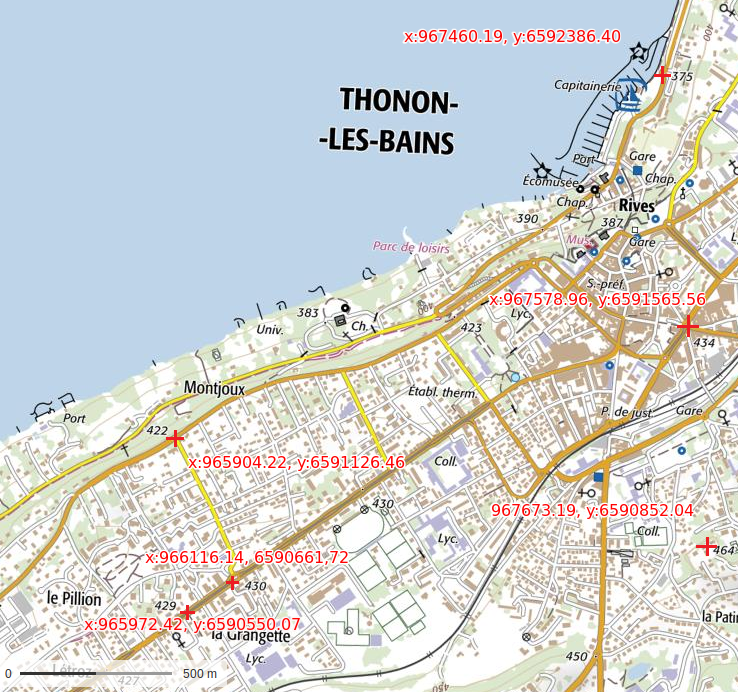
\includegraphics[height=2.5cm,width=2.5cm]{images/georeferencing/ign-points-Thonon.png}
\end{overlayarea}
\begin{overlayarea}{\linewidth}{2cm}
  \centering
  \scriptsize IGN image georeferenced in $Lambert$ $93$ system\par
\end{overlayarea}
\end{column}
\begin{column}{0.30\textwidth}
%\begin{overlayarea}{\linewidth}{0.0cm}
%  \centering
%  \par
%\end{overlayarea}
\begin{overlayarea}{\linewidth}{3cm}
  \centering\vfill
  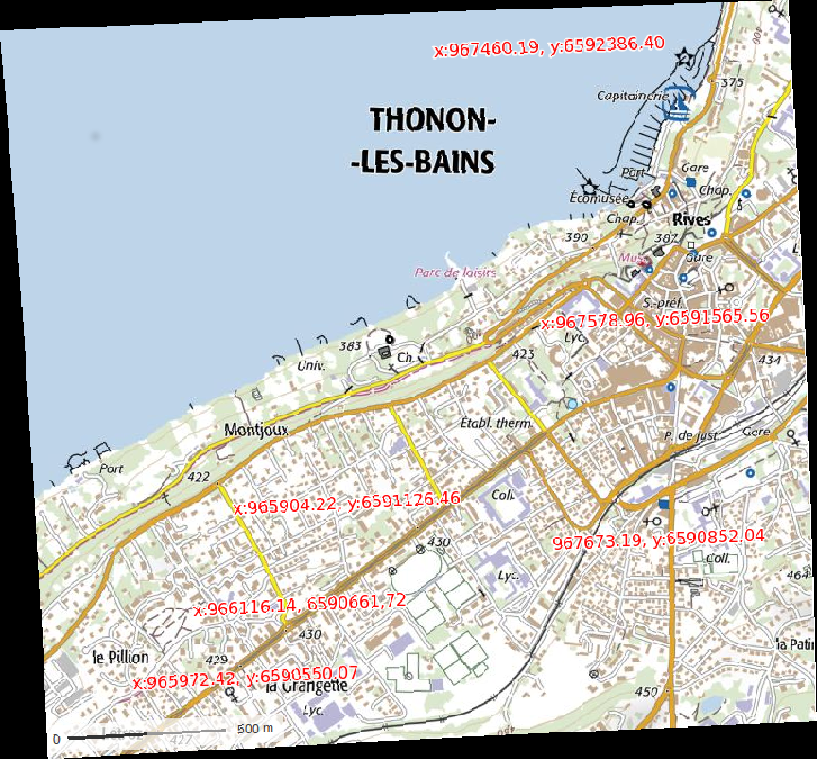
\includegraphics[height=2.5cm,width=2.5cm]{images/georeferencing/qgis-resultat.png}
\end{overlayarea}
\begin{overlayarea}{\linewidth}{2cm}
  \centering
  \scriptsize Then IGN image is tranformed to be georeferenced in $UTM$ system\par
\end{overlayarea}
\end{column}
\begin{column}{0.30\textwidth}
%\begin{overlayarea}{\linewidth}{0.0cm}
%  \centering
%  \par
%\end{overlayarea}
\begin{overlayarea}{\linewidth}{3cm}
  \centering\vfill
  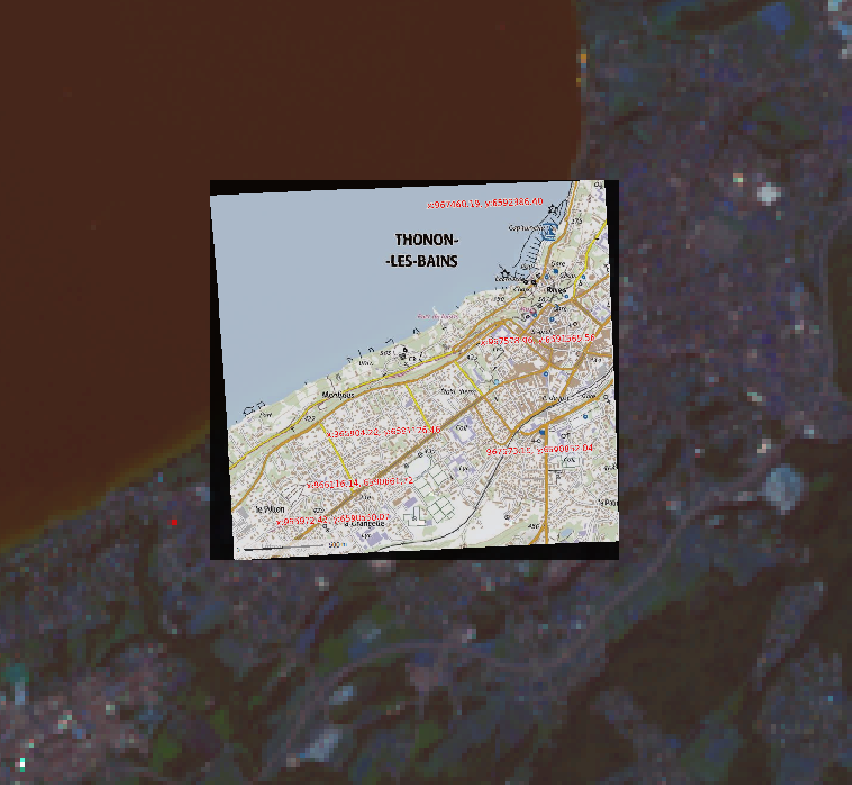
\includegraphics[height=2.5cm,width=2.5cm]{images/georeferencing/qgis-superposition0.png}
\end{overlayarea}
\begin{overlayarea}{\linewidth}{2cm}
  \centering
  \scriptsize Superposition of IGN and Landsat-8 images both georeferenced in $UTM$ system\par
\end{overlayarea}
\end{column}
\end{columns}

\end{frame}

\section{Importing Data}

\subsection{Image query}
\begin{frame}
 \begin{itemize}
 \item Query images from \href{https://earthexplorer.usgs.gov/}{\begin{itshape}U.S geological Survey\end{itshape}} website
 \begin{itemize}
  \item cloud covering \ 20\%\\
  \item day acquisition\\
  \item between May, 2013 and September, 2013\\ 
 \end{itemize}
 
\end{itemize}

\begin{columns}[t]
\begin{column}{0.50\textwidth}
\begin{overlayarea}{\linewidth}{4cm}
  \centering\vfill
  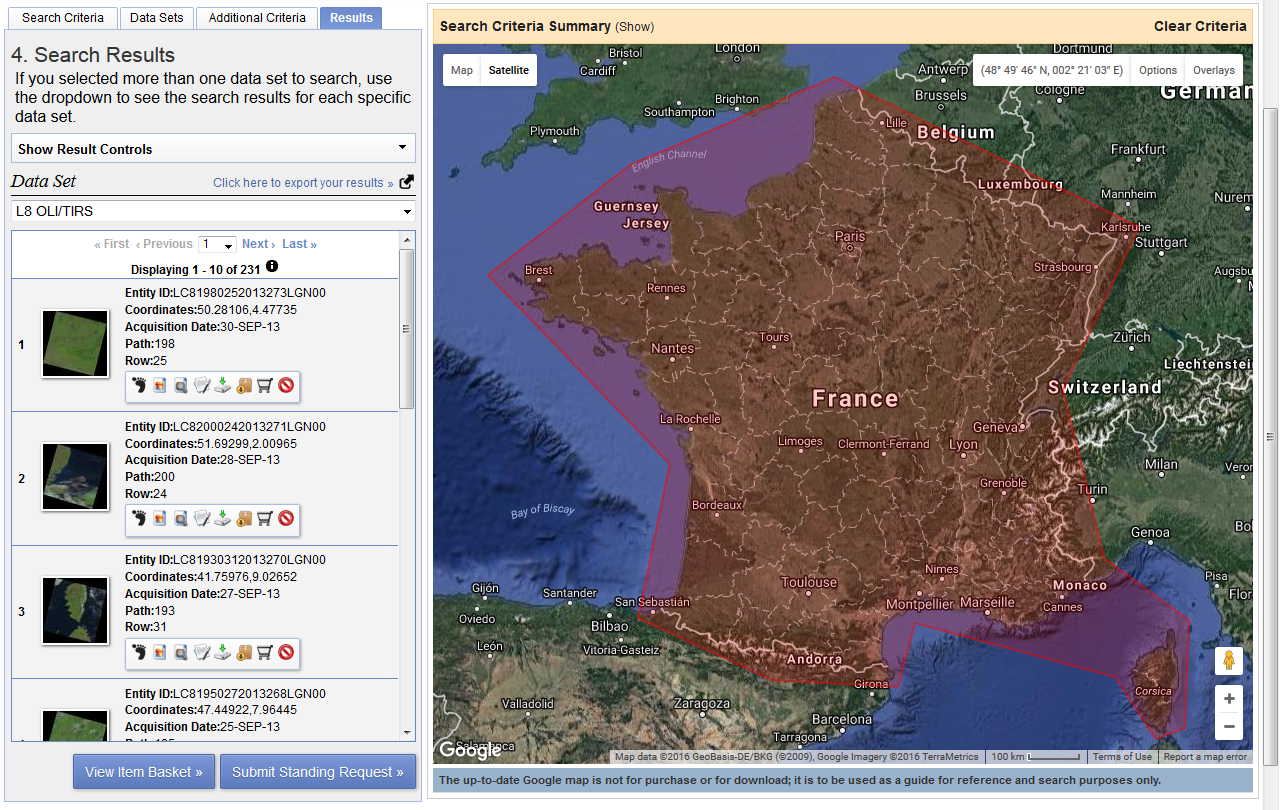
\includegraphics[scale=0.17]{images/importing/france-selection.png}
\end{overlayarea}
\begin{overlayarea}{\linewidth}{1cm}
  \centering
  \scriptsize Polygon selection on $USGS$ website\par
\end{overlayarea}
\end{column}

\begin{column}{0.50\textwidth}
\begin{overlayarea}{\linewidth}{4cm}
  \centering\vfill
  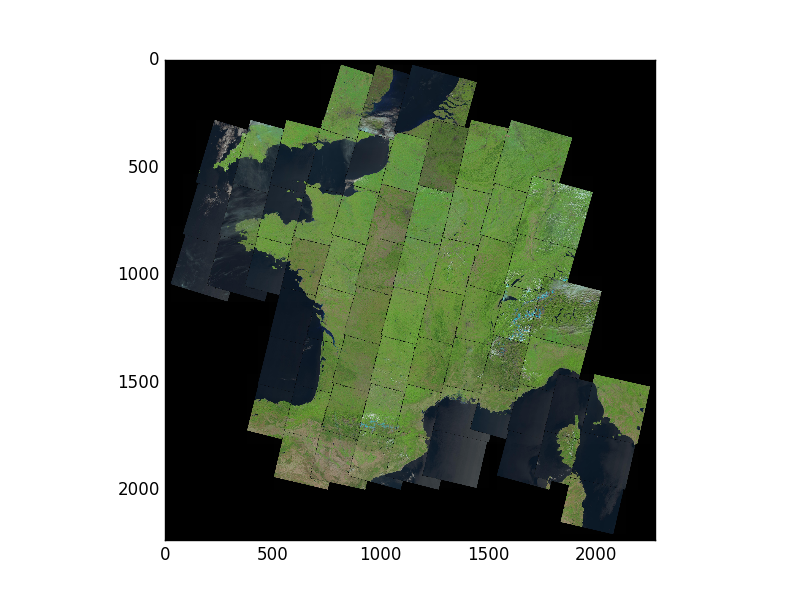
\includegraphics[scale=0.25]{images/importing/france-covering.png}
\end{overlayarea}
\begin{overlayarea}{\linewidth}{1cm}
  \centering
  \scriptsize Resulted images georeferenced in $UTM$ system\par
\end{overlayarea}
\end{column}
\end{columns}

\end{frame}

\subsection{Image bands}
\begin{frame}
 
\end{frame}

\section{Importing labels}
\begin{frame}
 
\end{frame}

\section{Vegetation index extraction}

\subsection{NDVI extraction}
\begin{frame}

\end{frame}

\subsection{NDVI evolution}
\begin{frame}

\end{frame}

\subsection{Data to Machine Learning}
\begin{frame}
 
\end{frame}

\section{Supervised Regression}
\begin{frame}

\end{frame}

\section{Supervised Classification}
\begin{frame}

\end{frame}

\end{document}
